% !TEX root = _main.tex
% \title{合成音声に朗読表現を付加するシステムの検討}
% \author{32145042　小山　実生}{KOYAMA Mio}{FUKU}[]



% ==========================================
% ここから本文．あとは各自で
% ==========================================

%1
\section{はじめに}

人々は言葉をもってコミュニケーションを行っているが、人が話す言葉には、文章自体の情報と発話された音声が含まれている。そのうち音声の部分は、文章のみでは伝わりにくい曖昧な部分を音で固定・補完をする役割をもっている。例えば「頭が赤い魚を食べる猫」\cite{twitter}という文章があった場合、文章に対し音の区切りや抑揚を適切につけることで「頭が赤い」のは「猫」なのか「魚」なのかが分かりやすくなる。また、音声の抑揚や強さ、速さを調節することで情報伝達だけでなく、話者の感情や解釈を伝えることができる。例えば「成功して良かったね」という文章に対し、はつらつと読むと嬉しそうな印象が伝わるが、平坦に読むと冷たい印象が伝わる。このように、人の発話には豊かな表現力が備わっている。

人の発話による音表現のひとつに朗読がある。朗読は報道機関でのアナウンスや公共施設での音声案内とは違い、情報伝達だけではなく音の表現にも重きを置かれる。そのため、朗読には音を鑑賞する測面も持ち合わせているとも考えられる。同じ文章でも、異なる話者が読み上げると全く違う発話表現が為されているからこそ、数多くの声優やナレーターが存在し、同じ演目の朗読劇が何度も催されているのではないだろうか。

本研究では、同じ文章でも異なる音の表現を生み出し、朗読のような発話表現に重きを置かれた音声を作りだせるシステムを作りたいと考え、既存の合成音声生成ソフトウェア『VOICEPEAK[2]』をベースにPythonにてシステム構築を行った。また、ユーザに「間」の置き方を対話形式で選択させることで、出力される音声の多様化を図った。



%2

\section{音を通じたことばの表現}
\subsection{文章表現の曖昧さ}
ことばは、情報を的確に・時空を超えて・遠く・大勢に伝えるための記号として、人間社会の中で言語が発展し体系化された。そのことばの表現には、その自体の内容を伝える「情報」と発話された「音」の二つが含まれているが、一般的には、ことばの表現には情報が正しく伝わる文章力の側面が強く重視される。その一方で、文章のみでは文脈が伝わりにくい状況も時に発生する。文脈がややこしくなる文章を伝えやすくする文章上の工夫にはどのようなものがあるだろうか。

(1) 言葉の係り受けの整理

係り受けとは、日本語の文法において、単語や文節がどのように関係し合い、文全体の意味を構成するかを示す概念である。具体的には、「係り」成分(修飾語)と「受け」成分(被修飾語)の関係を整理することで、文章の構造や意味を明確にする。頭が赤い魚を食べる猫\cite{twitter}という文章に対し、どこまでが「係り」成分でどこからが「受け」成分なのかを分析することで、文章が持つ意味を明確にすることができる。

(2)句読点や行間の工夫

日本語は漢字、ひらがな、カタカナが混在した言語であるため、情報量が多くなる。そこで句読点や行間を文章に折り込むことで文字の密集を防ぎ、視覚的に読みやすくする。また、段落や内容の変わり目を分かりやすくする効果も期待できる(\figref{fig:redcat1})。


\begin{figure}[tb]% h ではなくt(op)かb(ottom)で
    \centering
    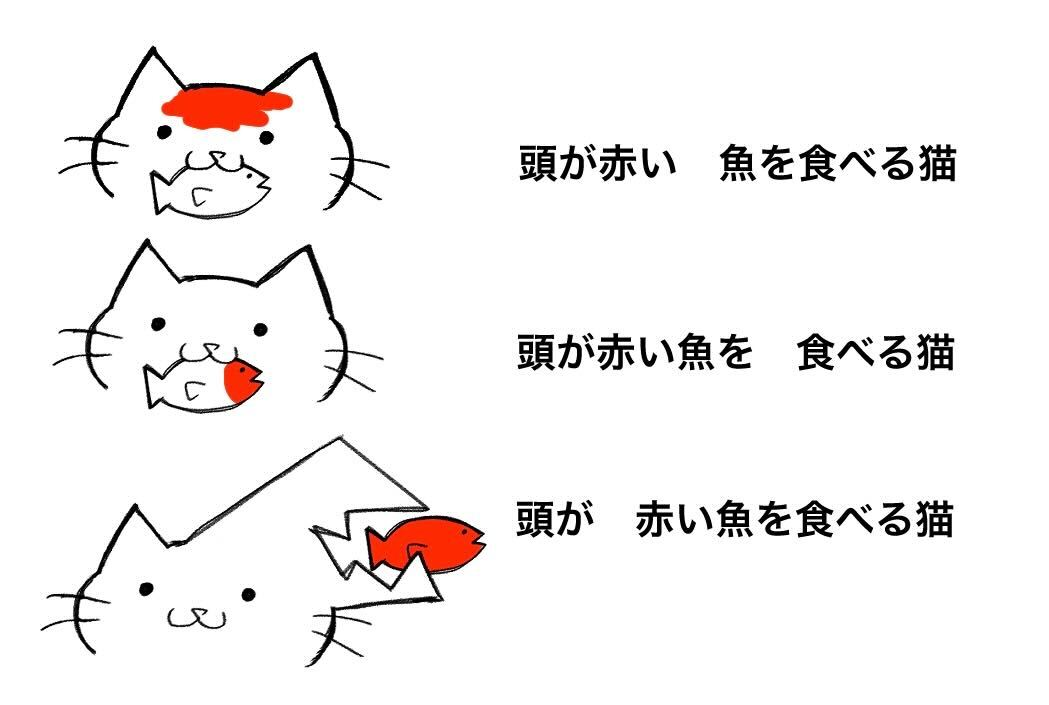
\includegraphics[width=\hsize]{fig/osakana.jpg}
    \caption{音で伝える「頭が赤い魚を食べる猫」（{文献\cite{akaineko}を元に筆者作成}）}
    \label{fig:redcat1}
\end{figure}


\subsection{発話制御による自然な情報伝達と感情表現}
人々はコミュニケーションをとるうえで、文を音に乗せて発話することで相手に情報を伝える。発話された音声には、文章自体の内容を伝える「情報」と発話された「音」の二つが含まれている。このうちの「音」には、文章のみでは伝わりにくい曖昧な部分を固定・補完する役割を持っている。

例えば「頭が赤い魚を食べる猫」という文章\cite{twitter}では，文章のみであると、「頭が赤い」という単語はどの名詞を説明しているのかが一見分かりにくい。また、「食べて」いるのは「猫」ではなく「猫の頭」という解釈もすることができる。こういった複数の解釈が生まれかねない文章に対し、音の区切りや抑揚等の「音」を適切に付随させることで、「赤い頭」をしているのは「猫」なのか「魚」なのか、はたまた「食べる」のは「猫」なのか「猫の頭」なのかが相手に伝わるようになる。このように、「音」には文章を固定・補完させる役割があると考えられる。


また、人の発話による音声表現の塩梅は、話者によってかなり変わってくる。\figref{fig:1}は、全く同じ文章を読み上げている、異なる話者(いずれも男性)による朗読音声\cite{Kubota,Torikai21}をスペクトログラムで表したものである(\figref{fig:1})。


\begin{figure}[tb] % h ではなくt(op)かb(ottom)で
    \centering
    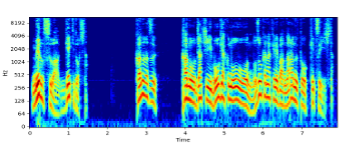
\includegraphics[width=\hsize]{fig/fig1a.png}
    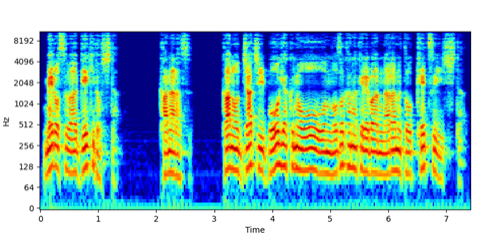
\includegraphics[width=\hsize]{fig/fig1b.png}
    \caption{異なる話者による『走れメロス』のスペクトログラム}
    \label{fig:1}
\end{figure}

これらはPythonのライブラリのひとつである『Librosa\cite{librosa}』を使って出力した。文章は、太宰治作『走れメロス\cite{Dazai}』の冒頭『メロスは激怒した。必ず、かの邪知暴虐の王を除かなければならぬと決意した。』という部分を読み上げている。スペクトログラムとは、音の高さ、音色、大きさ、長さといった音の四要素を表す短時間フーリエ変換の表示であり、図の横の長さが時系列、音の強さを濃淡、波形の動きが音高やその移り変わりを示している。これら二つの図から、同じ文章でも話者が変われば全く違う音声が生まれていることが分かる。

また、それぞれのスペクトログラムに波形の動きが途切れている箇所が二つあるが、それらは文章の合間の『、』と『。』の部分を表している。これらからも、話者によって文の合間をどのくらい空けるかが変わっている。つまり、間の持たせ方も話者の持つ表現や解釈によって変わるのである。同じ文章でも話者の表現や解釈ごとに朗読が変化するのである。


\subsection{音による感情の表現}
音声の発話表現には読む速さや高さ、抑揚、強さ、単語のイントネーションなど、多くの要素がある。これらを細かく適切に調節することで、正確な情報伝達だけでなく話者の感情や意思を伝えることができる。例えば、「成功して良かったね」という文章があったとする。この文章に対し、声を高くはつらつと読むと嬉しそうな印象が伝わり、話者もまた成功を喜んでいることを伝えられる。一方、抑揚をあまり付けず平坦に読むと冷たい印象になり、言葉裏に話者自体は「良かった」とあまり思っていない、もしくはどうでも良さそうなイメージを聞き手に伝えられる。
音声に含まれる感情には、コミュニケーションにおける話し手が実際に抱いている主観的なものと、感情表現を客観的に聞き手に共有されるステレオタイプの二つが考えられる\cite{sutereo}。そして、感情表現は日常におけるコミュニケーションだけでなく、音を豊かに表現する朗読においても重要な要素の一つとも言える。登場人物のセリフや心情などが描写された文章に感情的な表現を入れて読むことで、聞き手の物語に対する没入感がかなり変わる。





\subsection{話者による解釈違いを楽しむ朗読表現}\label{kaishaku}
%本研究では、同じ文章でもイントネーションやアクセント、間の置き方等の細かな表現を調節することで、異なる音声表現を作成するシステムの開発を行った。また、文章全体のイントネーションや速度、ポーズの長さを独自設定したものに一括変更させることで、デフォルトで生成されるものより表現力のある合成音声を出力させる機能を搭載した。次章では、文章を読み上げる合成音声生成ソフトウェアについて取り上げる。

ことばの表現のひとつに朗読がある。朗読の定義は様々だが、他者に文章内容を聞かせるために発音するものである。また、発声された文章によって、聞く者にイメージや情念を喚起させるようにいわゆる「表現として」読むことであるとも考えられている。つまり、音楽や美術の鑑賞と同じように、ただ聞き手に情報を与えるだけではなく、聞き手のこころに響かせるひとつの芸術として捉えられる。
筆者には朗読の経験があり、朗読表現をつけるために様々な練習をしていた。例えば、「あー」という音を一分間、同じ音量、音程、強さをキープしながら出し続ける練習だったり、外郎売\cite{uirou}を読んで滑らかに発声できるようにする練習など、朗読に向けて数多くの練習を行った。その中のひとつに、読み上げる原稿に対してブレスする箇所、間を空ける箇所を前もって決める作業があった。この作業をすることで、話者は息継ぎをする場所を決められたり、どの部分に余韻を持たせるかを考えることができる。
この考えを活かし，本研究ではユーザによって異なる朗読表現が作成されるシステムを構築した。

\section{関連研究：合成音声ツールの現状}
合成音声とは、コンピュータなどを用いて人間の発話を真似た音声を人工的に生成されたもので、任意の文章を音声に変換して様々なことを発話させることができる。コンピュータから作り出せる音声として、単語単位を録音して作り出せる録音編集方式や、子音と母音を繋ぎ合わせて出力する規則音声方式などがある。また近年では深層学習(DNN)に基づいた合成音声も開発\cite{Zen2013}され、発話の品質は高くなっている。

さらに、感情表現のついた合成音声に関する研究も進められており\cite{Ichikawa67,Hirose94,Iida99}、感情のついた合成音声を生成できるソフトウェア\cite{voicepeak,aivoice}やツール\cite{GPT-4o}も数多く存在している。
以下，既存のソフトウェアを用いてどれだけ朗読表現を行うことができるか，VOICEPEAK\cite{voicepeak}とA.I.VOICE2 Editor\cite{aivoice}を例に試行する．

\subsection{VOICEPEAK}

\begin{figure}[tb]
    \centering
    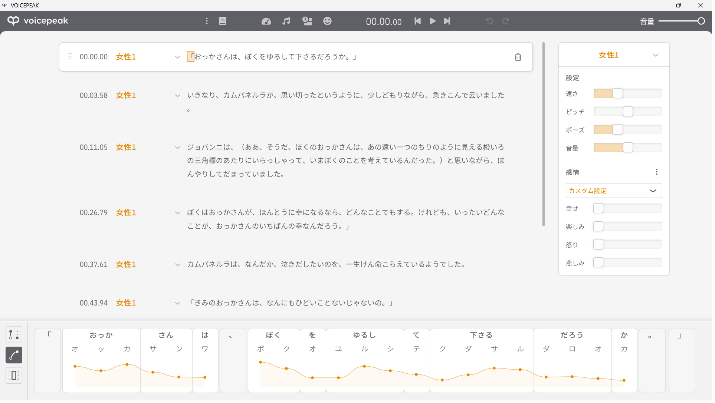
\includegraphics[width=\hsize]{fig/fig2-vp.png}
    \caption{VOICEPEAK}
    \label{fig:voicepeak}
\end{figure}


VOICEPEAK\cite{voicepeak}とは、株式会社AHSによって開発・提供されているTTS(text to speech)の合成音声生成ソフトウェアである(\figref{fig:voicepeak})。読ませたいテキストを入力するだけで合成音声を出力させることができる。また出力された合成音声の表現に不満があった場合でも、イントネーションやアクセント、読み上げる速さなどを自分好みに調節することができる。VOICEPEAKは、一音ごとのアクセント、イントネーション、音の区切り、長さなどの細かい調節も画面上に表示され、それらを直感的に操作することが可能である(\figref{fig:vpedit})。また、文章全体やブロック毎での読む速さやピッチも調節可能であり、感情表現(幸せ 悲しみ 怒り 楽しみ)も付随させることができる。そのため、豊かな表現力がついた合成音声を作成することが可能である。

\begin{figure}[tb]
    \centering
    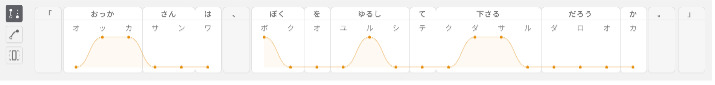
\includegraphics[width=\hsize]{fig/fig3a.png}
    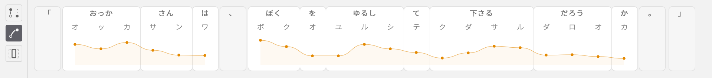
\includegraphics[width=\hsize]{fig/fig3b.png}
    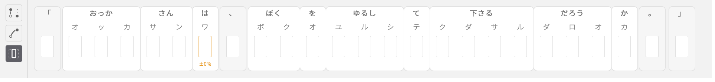
\includegraphics[width=\hsize]{fig/fig3c.png}
    \caption{VOICEPEAKのパラメータ表示}
    \label{fig:vpedit}
\end{figure}


\subsection{A.I VOICE2 Editor}

A.I.VOICE2 Editor\cite{aivoice}とは、株式会社エーアイが提供している音声合成ソフトである(\figref{fig:aivoice})。音声合成AITalk\cite{aitalk}の技術を応用した個人利用者向けソフトウェアで、テキストを入力するだけでキャラクターに自然な音声合成で読み上げられる。またそれらは音声ファイルとして保存することも可能である。テキストを読むキャラクターは数多く展開されており、声色を好みに合わせて選択・ダウンロードすることができる。このソフトウェアは、アクセントとイントネーションの調節はいっしょくたにされているものの、音声全体やブロック毎の音量や読む速さ、高さ、抑揚、感情表現などのパラメータを具体的な数値で入力できる(\figref{fig:aivedit})。また、キャラクター独自の話し方で他のキャラクターの声色で発話させることができる『ボイスフュージョン機能』もA.I.VOICE２の大きな特徴と言える。


\begin{figure}[tb]
    \centering
    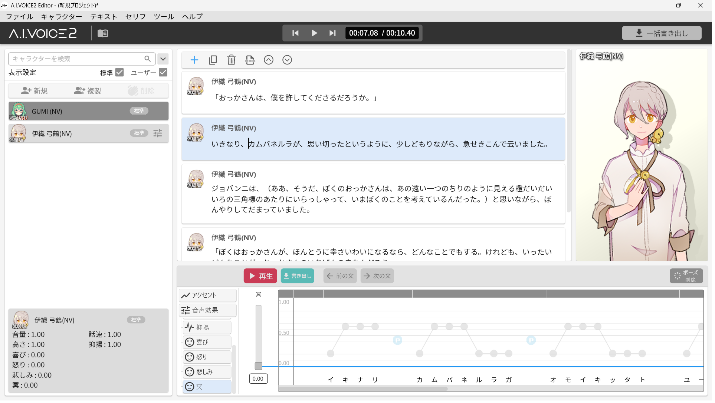
\includegraphics[width=\hsize]{fig/fig4-aiv.png}
    \caption{A.I VOICE2 Editor}
    \label{fig:aivoice}
\end{figure}

\begin{figure}[tb]
    \centering
    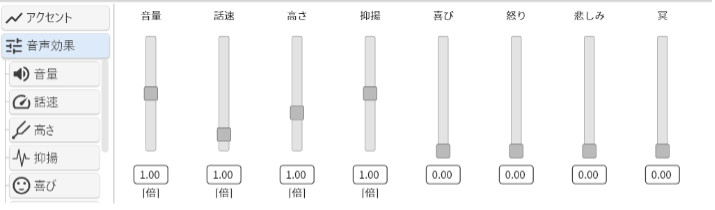
\includegraphics[width=\hsize]{fig/fig5-aivedit.png}
    \caption{A.I VOICE2 Editorのパラメータ表示}
    \label{fig:aivedit}
\end{figure}

\subsection{朗読表現制御の課題 }
%上記２つのソフトでも朗読表現は一応作れるはず．なのに自分は自作する．なぜ？...に答えるために，既存ソフトでの朗読表現の難しさについて語れ．「面倒くさい」の一言では不足．どうめんどくさいの．どのぐらい時間がかかるものなのか，どう手間なのか，どうなってくれてたらそれらが解消される（と期待する）のか？



%\subsection{VOICEPEAKの長所と課題点} ←こっちに移動
VOICEPEAKはテキストを入力するだけで、合成音声が自動で作成される。また、合成音声を手軽に作成するだけでなく、文章全体の感情や文章ブロックごとの感情調節、一音ずつのアクセント、イントネーション、音の区切り、長さを細かく指定することも可能であり、より豊かな表現力のついた合成音声を作成することができる。

しかし、音声表現をソフトウェア上から調節する場合、調節方法はマウスポインタ—をドラッグ・クリック操作で描写されたグラフやバーを直接動かすしか方法がない。つまり、一つ一つの調整をするのに時間がかかる。(\figref{fig:melos})。また、朗読をする話者によって、同じ文章を読んでいても間の作り方や区切り(ブレスの位置)が変わってくる。そのため、朗読表現に重きを置いた音声を作ると考えた場合、テキスト通りに書かれた句読点をそのまま読み上げるわけにはいかない。

また、A.I.VOICE2で音声を調整する場合、アクセントの指定はできるものの、文章全体のイントネーションの流れはシステム側で自動的に設定される(\figref{fig/AIVOICE.png})。そのため、表現に関して、ユーザに選択の余地を与えられている部分が少ない。

これらをふまえて、本システムではイントネーションやアクセントの出力はVOICEPEAKのシステムに任せつつ、話者によって大きく変わる間の区切りはシステムからの提案による対話形式でユーザに決めさせるように構築した。

\begin{figure}[tb]
    \centering
    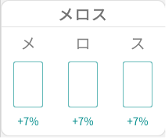
\includegraphics[width=.5\hsize]{fig/fig6-melos.png}
    \caption{ソフトウェア状でのパラメータ表示}
    \label{fig:melos}
\end{figure}

\begin{figure}[tb]
    \centering
    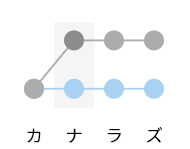
\includegraphics[width=.6\hsize]{fig/AIVOICE.png}
    \caption{A.I.VOICE2でのアクセントの指定}
    \label{fig:melos}
\end{figure}





\section{朗読表現支援システム}
本章では、自身が組んだシステムについて述べる。%\subsection{\red{本研究のアプローチ}}
本研究では、内部で作られるファイルの分かりやすさや理解のしやすさをふまえてVOICEPEAKを土台にシステム開発を行うことにした。そのため，
VOICEPEAKのソフトウェア\footnote{『VOICEPEAK 商用可能 ６ナレーターセット』，\url{https://xxx}}、及びVOICEPEAKによって作成されたvpp形式のファイルがデバイス上にあることを前提とする。

%本章では、VOICEPEAKについての挙動や作成されるファイルについて説明していく。本研究では、『VOICEPEAK 商用可能 ６ナレーターセット』という製品を使用している。



\subsection{システムの機能}
%\subsection{従来のVOICEPEAKとの相違}
本研究システムでは文章の間の取り方を対話形式で提案している。間の取り方については、６人の話者による朗読音声を参考に筆者が間の空け方を調べ、独自にデータ化したものから提案する(\figref{fig:kugiri})。これにより、ユーザ毎に異なる表現の多様化を図っている。また、全体的なピッチの高さ、読み上げる速さについては、システム側からおすすめの値の範囲を示したうえで、ユーザに設定してもらう。

\begin{figure}[tb]
    \centering
    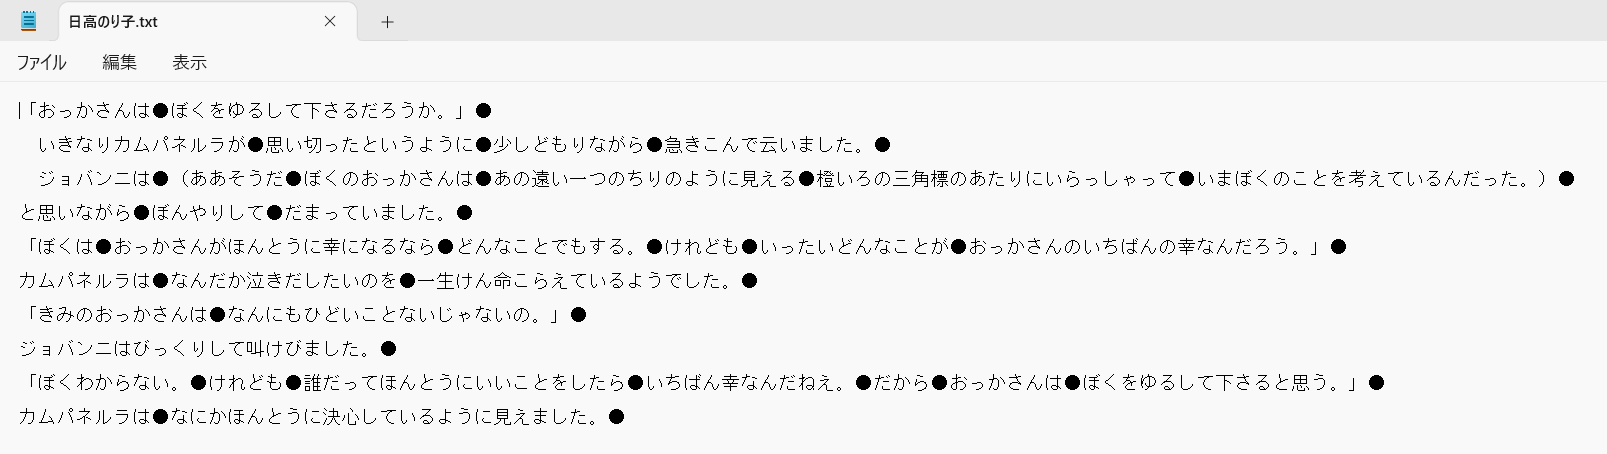
\includegraphics[width=\hsize]{fig/kugiri.png}
    \caption{筆者が独自に作成したデータの一部}
    \label{fig:kugiri}
\end{figure}



%「表現力」「細かく調節できる機能」とは，具体的になにしてるの？VOICEPEAKでできなかったことが，本システムではどうできるようになっているのか明確にする．表にしてもよい



\subsection{VOICEPEAKのデータ構造}
VOICEPEAK上で作成されたファイルは、vpp形式で保存される。vppファイルの実態はJSON形式であるため，Python上で直接的にファイルの入出力をすることが可能である。
%さらに、ファイル上に書かれた、各々のパラメータに対応する数値を変更することで、VOICEPEAK上で生成される合成音声の表現を調節することができた。そこでVOICEPEAK上で表示されるGUIからパラメータを操作し、保存した後に内部ファイルを開いてどの値が変化したのか手作業で調べることで、イントネーションやアクセント、長さがどの部分に対応するのかを解析した。

% 
% \begin{figure}[tb]
%	\centering
%	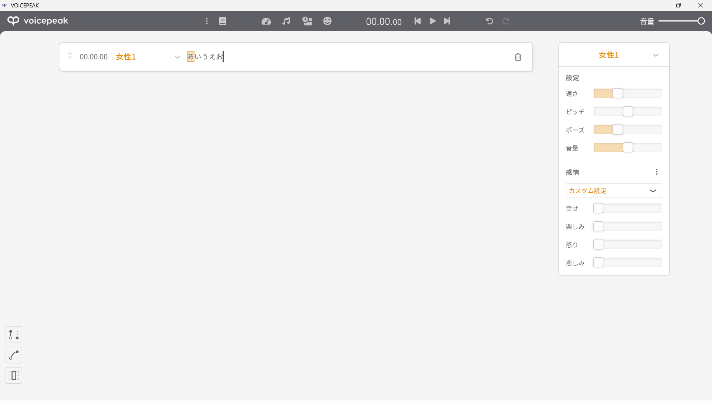
\includegraphics[width=\hsize]{fig/fig7-sys.png}
%	\caption{vppファイル}
%	\label{fig:sys}
%\end{figure}
%
%\begin{figure}[tb]
%	\centering
%	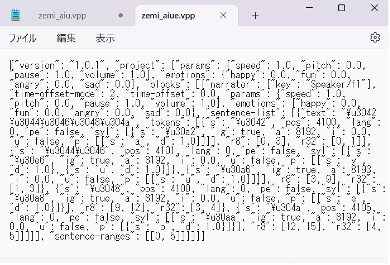
\includegraphics[width=\hsize]{fig/fig8-text.png}
%	\caption{vppファイルの内部}
%	\label{fig:text}
%\end{figure}


\begin{table}[htb]
    \centering
    \caption{voicepeak内部ファイルのキー}
    \begin{tabular}{c|l}\hline
        project         & プロジェクト全体に関わる設定が含まれる                   \\ \hline
        params          & 話者全体に共通する調整パラメータ                      \\
        speed           & 話速                                    \\
        pitch           & 音高                                    \\
        pause           & ポーズの長さ                                \\
        volume          & 音量                                    \\
        emotions        & 話者の感情パラメータ \scriptsize{(happy, angry, sad, など)} \\
        s               & トークンの文字列 (例: '銀河')                    \\
        pos             & 品詞情報 (例: 4096)                        \\
        lang            & 言語コード (例: 0)                          \\
        pe              & 省略形かどうか (例: False)                    \\
        syl             & 音節情報のリスト                              \\
        syllable data   & 音節ごとのデータ                              \\
        ig              & 音節が有効か (例: True)                      \\
        a               & アクセントの強弱 (8193: 強, 8192: 弱)           \\
        i               & ピッチの調整値 (例: 0.0; 範囲は -3.0～+3.0)       \\
        u               & 無声かどうか (例: False)                     \\
        p               & 音声要素のデータ (例: 子音や母音)                   \\
        sentence-ranges & 文中のトークンのインデックス範囲                      \\ \hline
    \end{tabular}
    \label{voipi}
\end{table}



%\subsection{vppファイルの解析}
%\figref{fig:text}は、\figref{fig:sys}をメモ帳から開いた場合に出てくるファイルである。これは「あいうえお」という文章を読ませるファイルである。ファイルの冒頭には”version”キーが含まれ、プロジェクトのバージョン情報が記載されている。次に含まれている”params”キーの下には音声速度(speed)、音程(pitch)、ポーズの長さ(pause)、音量(volume)などの設定が格納されており、これはテキスト全体の調節をすることができる。また、”emotions”キーでは４つの感情表現を設定することができる。”narrator”キーでは声色の設定ができる。
%二回目以降に出てくる音声速度(speed)、音程(pitch)、ポーズの長さ(pause)、音量(volume)、表情(emotion)は、ブロック毎に括られているテキストの音声を調節することができる。
%“text”は打ち込まれた文章をエスケープシーケンスで格納している。さらに、”tokens”にて1-2音ずつの情報を格納しており、これらにパラメータが設定されている。この中にアクセント、イントネーション、音の長さの情報も含まれており、アクセントは8192 8193 4096のいずれか、イントネーションは-3から3の値、長さは正の値で管理されている。(分かりやすく表を示したい)


%\subsection{システム実装に向けて}
これらの結果をふまえ、本システムではvppファイル内に含まれているテキスト部分を、対話形式によって手に入れたユーザの入力情報に書き換えて保存することで、Python上からVOICEPEAKの合成音声の表現(間の区切り)を変えられるようにした。

\subsection{処理の流れ}

\begin{figure}[tb]
    \centering
    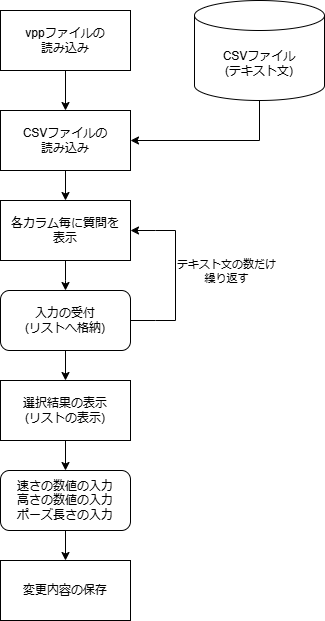
\includegraphics[width=.7\hsize]{fig/fig10_flow.png}
    \caption{システムのフローチャート}
    \label{fig:flow}
\end{figure}


本システムは，コマンドラインで稼働するCUIシステムとして実装している。

\subsubsection{ファイルの読み込み}
まず、vpp形式のファイルをjson形式に変換し、オリジナルに含まれている不要な末尾の文字を削除する。これをすることで読み込む際にエラー表示がされなくなる。また、対話形式で表示させるテキストが格納されているCSVファイルをここで読み込んでいる(\figref{fig:csv1})。

\begin{figure}[tb]
    \centering
    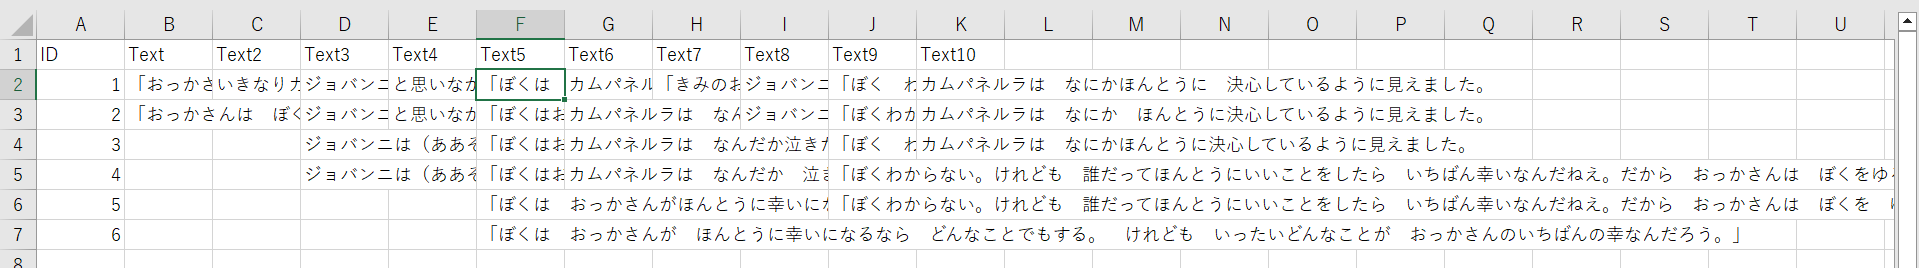
\includegraphics[width=\hsize]{fig/csv1.png}
    \caption{CSVファイル}
    \label{fig:csv1}
\end{figure}

\subsubsection{質問の表示・入力受付}
CSVファイルに格納されている、ブロック毎のテキストをターミナルに表示させる(\figref{fig:sys23})。ここで、ユーザに対話形式でお好みのテキストを選択してもらう。また、表示される異なる区切りのテキストは、６種類の朗読音声を参考にして筆者が作成したものである。これを、テキスト文の数だけ繰り返し行う。

\begin{figure}[tb]
    \centering
    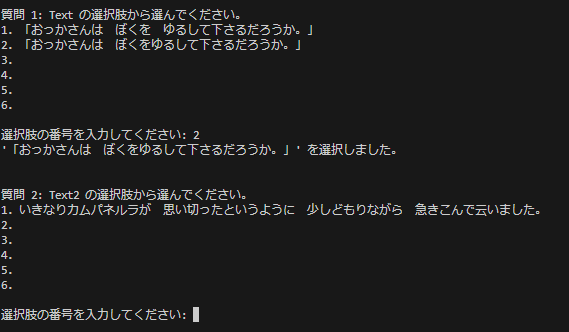
\includegraphics[width=\hsize]{fig/sys2.3.png}
    \caption{システムの表示画面１}
    \label{fig:sys23}
\end{figure}

\subsubsection{選択結果の表示}
繰り返しが終了すると、ユーザが選択したテキストが表示される(\figref{fig:sys22})。

\begin{figure}[tb]
    \centering
    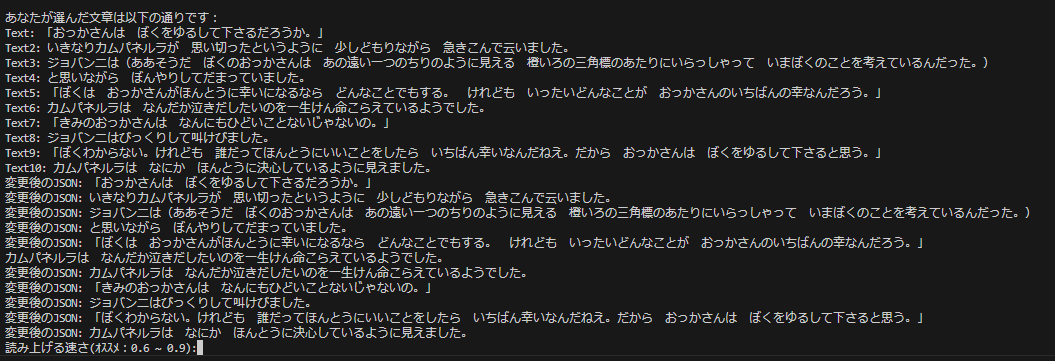
\includegraphics[width=\hsize]{fig/sys2.2.png}
    \caption{システムの表示画面2}
    \label{fig:sys22}
\end{figure}

\subsubsection{全体の高さ・速さ・ポーズの長さの設定}
その後、音声の全体的な設定へ移る(\figref{fig:sys21})。ユーザに各々おすすめの値の範囲を示したうえで、好みの値を入力してもらう。入力が終わると、vppファイルが設定したように書き換えられ、保存される。


\begin{figure}[tb]
    \centering
    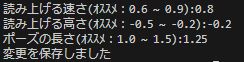
\includegraphics[width=.7\hsize]{fig/sys2.1.png}
    \caption{システムの表示画面3}
    \label{fig:sys21}
\end{figure}




% % ↓表記通りに出力させるためのもの．本文執筆時には削除すること
% \begin{verbatim}

% \end{verbatim}	% ------------ ←本文執筆時には削除

\section{適用事例}
\subsection{対象作品}
本研究システムによって音声に朗読表現がついたか確かめるために、分析対象を決めた。分析対象とするテキストは、宮沢賢治作『銀河鉄道の夜[16]』から引用したものに決定した(\figref{fig:ginga})。選定理由として、登場人物の心情描写や台詞、人物同士の対話が程よく含まれていると感じた。また感情の移り変わりがある描写も含まれており、朗読らしい表現が現れやすいテキストであるとも考えた。

\begin{figure}[tb]
    \centering
    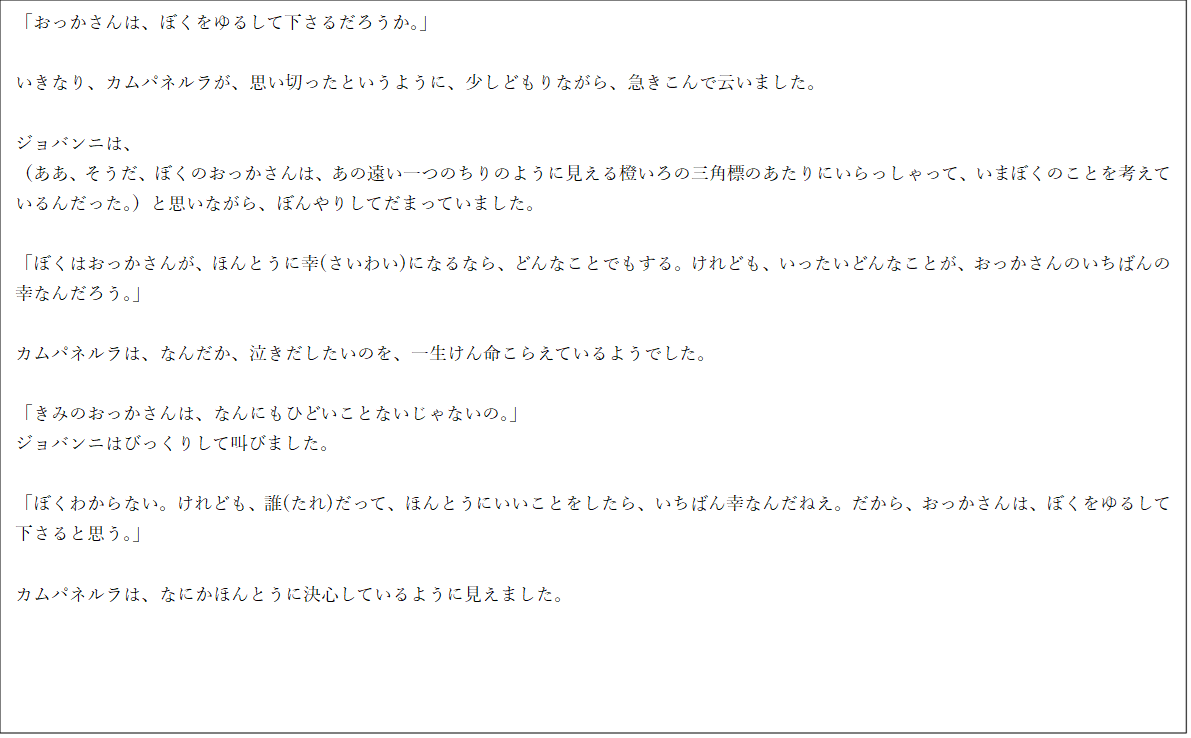
\includegraphics[width=\hsize]{fig/ginga.png}
    \caption{分析対象のテキスト}
    \label{fig:ginga}
\end{figure}

\subsection{手順}
まず、VOICEPEAK上にてテキスト入力をし、デフォルトのまま出力される合成音声を作成した。次に、本研究システムにて構築した一括変換機能にファイルを通し、保存されたvppファイルから合成音声を出力した。さらに、これらの音声を聞いたうえで、筆者が気になった部分のみを手作業で調節した。これらの音声はゼミ研究室が持つyoutubeのアカウントにて公開する。

\subsection{一部のイントネーションの変更}
VOICEPEAKによって出力されるイントネーションは、大部分はそれなりに上手く朗読的にふさわしいものとなっていた。しかし、Text6の「一生けん命」という部分がなぜか自然的な発音ではなく、聞いていて最も違和感の目立つ発音となっていた。そこで、Text6の部分のみ、筆者が６つの朗読音声を耳で聴きながら６つのvppファイルを作ることで、イントネーションのパラメータを作成した。それらの平均値を適応させることで、違和感を軽減させた(\figref{fig:ave})。



\begin{figure}[tb]
    \centering
    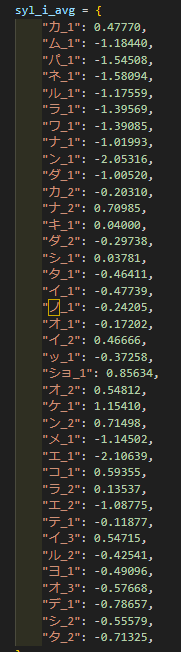
\includegraphics[width=.4\hsize]{fig/ave.png}
    \caption{Text6の平均値}
    \label{fig:ave}
\end{figure}




\subsection{朗読表現の簡易な操作}%はどの程度できたのか
%{自作する理由はここにあったはず．どれだけ「朗読」のために便利になったのか，事実を元に主張してみせるべし}
このシステムによって、朗読に触れたことのないユーザでも対話形式でテキストと３つの数値を選んでもらう操作のみで朗読っぽい音声を作り出すことができている。
\subsection{複数解釈による朗読表現}%はどの程度できたのか
%{\ref{kaishaku}節で，朗読は複数話者の解釈で色々表現変わるんだと主張している以上，実際それをシステムでやってみるべし．}
このシステムによって作成できる朗読音声のパターンは11250種類である。そのひとつひとつに大きな変化はなくとも、朗読特有の、話者によって変化する表現の多様化を再現できていると考えられる。
%上記までの修正に合わせて整える
\section{まとめ}朗読のような表現力のついた音声を、対話形式の選択と３つの数値の選択で出力できる合成音声システムを構築した。高い表現力とまではいかなくとも、朗読表現の差別化を図ることができた。
%上記までの修正に合わせて整える

本研究では、VOICEPEAKを土台としたうえで、豊かな表現のついた音声を出力するシステムの構築を図った。その結果、従来より豊かな表現力のついた合成音声を作り出すことができた。また、提供されているVOICEPEAK上での不満点を本研究システムにて解消するように努め、その結果、VOICEPEAK上では分からなかったパラメータ数値の表示をすることができ、より具体的な表現を指示ができるようになった。
一方、vppファイルの書き換えのみではどうしてもできない部分も浮き彫りになった。例えば、内部ファイルのみでは作られている音声の再生が不可能であり、ユーザにフィードバックを与えられない点などが大きな課題点として挙げられた。また、短ポーズ(「、」)と長ポーズ(「。」)の区別が上手くいかず、全体でポーズの長さを設定するときは一律で変更されてしまう点なども挙げられた。



% \section{おわりに}
% 謝辞
% \begin{acknowledgment}
%     %本稿の執筆にあたり，参考文献に挙げた方々のWebサイト，スライド，各種資料を大いに参考にさせていただいた．
%     書くならお好きに
% \end{acknowledgment}

